As described in the introduction in Chapter~\ref{ch:1_introduction}, the Power model is an ensemble model, consisting of a rule-based and a text-based component, whose goal is the comprehensible prediction of new facts. Given a query entity with a few known facts and descriptive texts, Power implements this requirement by providing prioritized lists of rules and sentences that were crucial for the predicted facts. Considering the application scenario in which a user uses the model for support of manual knowledge graph completion, it is also important that correct predictions are ranked as high as possible among an entity's predicted facts.

Technically, the Power ensemble consists of three components as shown in Figure~\ref{fig:4_approach/power_architecture}. Besides the rule-based component, named \emph{Ruler}, and the text-based component, named \emph{Texter}, it also contains the so-called \emph{Aggregator} that combines the Ruler's and Texter's predictions. If both Ruler and Texter predict a fact, the final prediction yielded by the Aggregator comes with both, the Ruler's prioritzed list of decisive rules and the Texter's ranked list of sentences, and is considered more reliable than a fact predicted by only one of the components.

\begin{figure}[t]
    \centering
    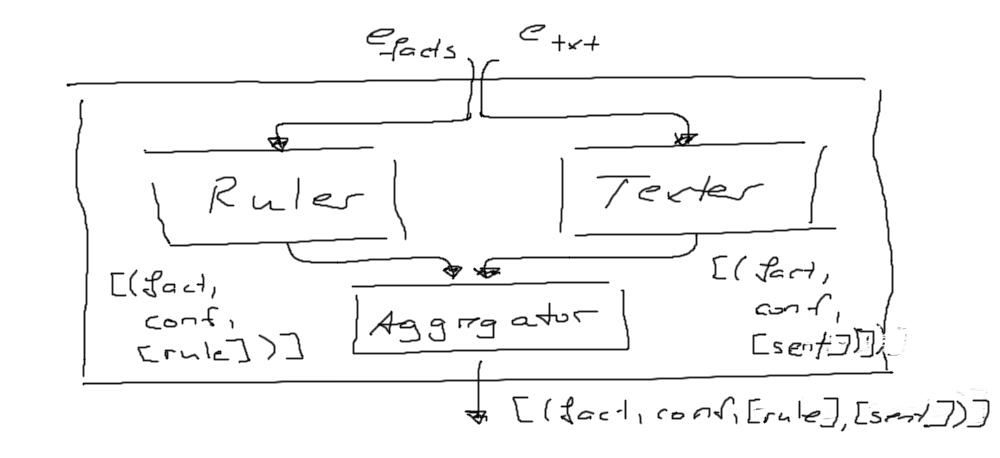
\includegraphics[width=\textwidth]{4_approach/power_architecture}
    \caption{Power model consisting of the Ruler, which processes a query entity's known facts, the Texter, which processes its texts, and the Aggregator, that combines all predictions; All predictions are sorted by confidence and come with sorted lists of explaining rules and texts}
    \label{fig:4_approach/power_architecture}
\end{figure}

Depending on the dataset at hand, either the Ruler or Texter might perform better. In general, the Texter should perform better for graphs that contain many similar facts, such as $(x, part~of, Asia)$ with $x \in \{China, India, Japan, \dots\}$, while the Ruler also works well on diverse datasets but cannot handle open-world entities about which no facts are known. Together, they complement each other: The Ruler handles very rare facts while the Texter can bootstrap the prediction process on open-world entities until the Ruler can join when some facts are available for rule application. In Chapter~\ref{sec:5_experiments/6_aggregator}, the Ruler's and Texter's evaluation results are compared to each other as well as to the results achieved by the Aggregator.

\section{Texter}
\label{sec:4_approach/1_texter}
While the Ruler processes the query entity's known facts, the Texter takes the entity's sentences to predict facts. Although it can only predict the most common facts from the training set, its main advantage is its applicability to open-world entities that come without any known facts about them.

\subsection{Simple Model}
\label{subsec:4_approach/1_texter/1_simple_model}
During inference, the first step of processing a query entity, which is the same for both the simple and the attentive Texter, is embedding the entity's sentences in the embedding block. Thereby, each sentence is processed individually as illustrated in Figure~\ref{fig:4_approach/1_texter/1_simple_model/simple_architecture}: First, the sentence is split into words by the tokenizer, which are handled as integer IDs in further processing. Next, the words are embedded using some NLP approach, which could be a simple lookup table in the simplest case. As the last step in the embedding block, the word embeddings are combined to sentence embeddings in the pooling layer. The resulting sentence embeddings, that capture the sentences' overall meanings, are then passed on to the classification block where each of them is pushed through the neural multi-label classifier which consists of a single linear layer. Another pooling layer then combines the sentence-wise classification logits to the entity's logits. Finally, applying the sigmoid function to the entity's logits yields the class probabilites that state the probabilities of the associated facts about the query entity.

\begin{figure}[t]
    \centering
    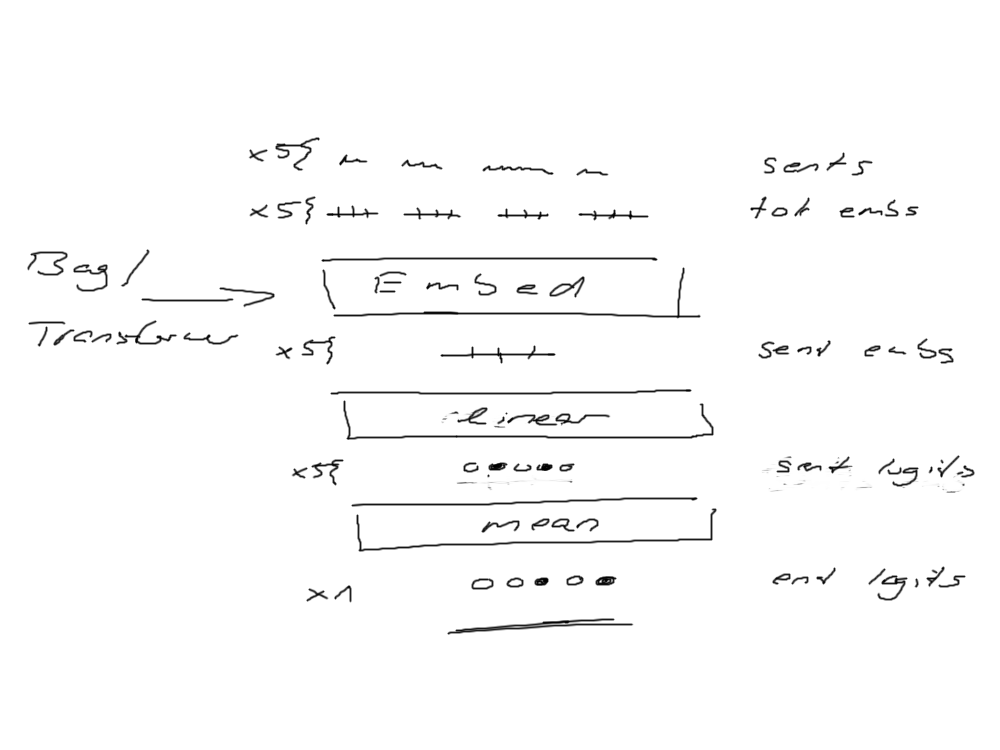
\includegraphics{4_approach/1_texter/1_simple_model/simple_architecture}
    \caption{Simple Texter Architecture; Each sentence is embedded and classified individually before the final pooling layer combines the results; "++++----" represents an embedding with positive and negative elements}
    \label{fig:4_approach/1_texter/1_simple_model/simple_architecture}
\end{figure}

Especially in the embedding block there are different possibilities for the concrete implementation of the individual parts to choose from, some of which will be examined in Chapter~\ref{ch:5_experiments}. In the final version of the power model, a transformer model is used for embedding the sentences' words, more precisely DistilBERT, a "distilled" variant of the transformer encoder BERT reduced to the essentials~\cite{Sanh2019DistilBERTAD}. In contrast to a simple lookup table, DistilBERT is able to incorporate the context of a word into its embedding, which leads to more meaningful sentence embeddings. This choice of embedding approach also affects the tokenizer, the pooling layer, and even the input sentences: Thanks to context embedding, transformers can use special tokens that add additional information to the text. While a classical model cannot decide on the basis of the sentence "Lisa likes John." whether this sentence speaks for the class $(x, has~gender, male)$, a transformer is able to do so given the appropriately marked sentence "Lisa likes [START]John[END].". Especially for long, ambigious sentences performance can be increased significantly.

Beyond the input data, the use of a transformer also affects the tokenizer and the pooling layer. The tokenizer has to apply byte pair encoding (BPE) that is commonly used by pre-trained transformers, where sentences are not only divided into words, but words are further divided into subwords, thus keeping the vocabulary of the tokenizer small and allowing to exploit homorphisms between similar words. In addition, the tokenizer inserts the [CLS] and [SEP] introduced by BERT at the beginning and end of the sentence. That way, "Lisa likes [START]John[END]." becomes "[CLS]Lisa likes [START]John[END].[SEP]". While the [SEP] token is used to separate sentences and has no further meaning here, the embedding of the [CLS] token captures the meaning of the whole sentence and is therefore  used as a sentence representation in the BERT paper~\cite{Devlin2019BERTPO}. However, the power experiments showed that performance can be increased if the word embeddings are also included, which is why the pooling layer of the embedding block averages all of a sentence's token embeddings, including the [CLS] embedding.

Less comprehensive processing steps happen in the classification block of the simple Texter: The sentence embeddings produced by the embedding block are pushed through the single linear classification layer whose multi-label output logits are averaged in the final pooling layer. The class probabilities calculated by applying the sigmoid function to the resulting entity logits are then used to sort the facts that have a probability greater than 50\%. Thus, the user of the model first receives the facts that are most likely to apply.


\subsection{Attention Model}
\label{subsec:4_approach/1_texter/2_attention_model}
While the simple Texter produces good evaluation results and does return a prioritized list of predicted facts, its prediction miss the desired explanation of why a fact is suggested. At this point, the attentive Texter extends the simple model by an attention mechanism that compares an entitiy's sentences to each other, forcing the model to favor sentences that are most relevant to the prediction of a certain fact. Besides the ability to provide an explanations for its predictions, the added attention mechanism should also increase the Texter's performance on datasets with multiple sentences per entity.

Technically, the attention mechanism is implemented as an attention block between the embedding and the classification blocks as shown in Figure~\ref{fig:4_approach/1_texter/2_attention_model/attention_architecture}. The embedding block is the same one used in the simple model, leveraging the DistilBERT encoder's contextual word embeddings to support marked input sentences and produce meaningful sentence embeddings. The classification block still produces the entity's multi-label output logits, but now uses multiple smaller linear layers to do so, due to the different outputs passed in from the attention block.

\begin{figure}[t]
    \centering
    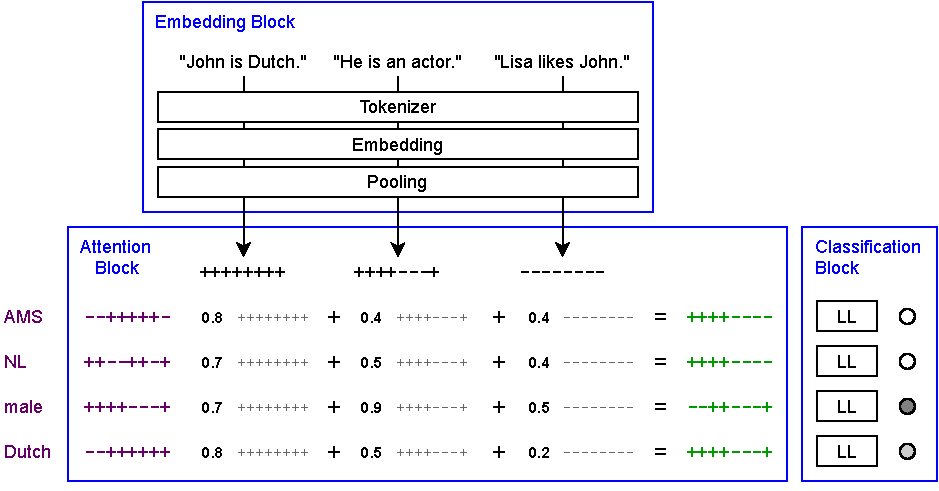
\includegraphics{4_approach/1_texter/2_attention_model/attention_architecture}
    \caption{Texter Architecture}
    \label{fig:4_approach/1_texter/2_attention_model/attention_architecture}
\end{figure}

The attention block now takes the sentence embeddings from the embedding block and compares them to so-called \emph{class embeddings} that represent each of the models output classes as a vector of the same dimension as the sentence embeddings. Given the set of input sentences $S$ and the set of classes $C$, the similarity between a class embedding $class_c$ and a sentence embedding $sent_s$ with $1 <= c <= |C|$ and $1 <= s <= |S|$ is calculated as the scalar product $\langle class_c, sent_s \rangle$ between the class and the sentece embedding. Given all class-sentence similarities for a certain class, the model can decide which sentence is matches the best for that class and deserves most attention when it comes to the decision whether the class holds true. Therefore, those similarity values are also referred to as attention values. To minimize the effect of sentences whose embeddings are very similar to a class embedding by pure chance, the attention values are furthermore normalized using the sigmoid function. Thus, the total attention matrix containing the attention values for all combinations of classes from $C$ and sentences from $S$ is calculated as shown in Equation~\ref{eq:4_approach/1_texter/2_attention_model/attention_matrix}.

\begin{align}
    A_{cs} = \sigma(\langle class_c , sent_s \rangle) && 1 <= c <= |C|, 1 <= s <= |S|
    \label{eq:4_approach/1_texter/2_attention_model/attention_matrix}
\end{align}

In the next step, the calculated attention values are used to combine the sentence embeddings to class-wise entity embeddings $ent_c$. As illstrated in Figure~\ref{fig:4_approach/1_texter/2_attention_model/attention_architecture} and formalized in Equation~\ref{eq:4_approach/1_texter/2_attention_model/ent_emb}, each sentence is thereby weighted by its class-wise attention value. The weighted sentences are then summed up to form class-wise entity embeddings whose purpose is to capture primarily those texts most relevant to the prediction of the respective class. Different from the simple Texter, the entity embeddings are then passed to the subsequent classification block instead of the original sentence embeddings.

\begin{align}
    ent_c = \sum_{s = 1}^{|S|} A_{cs} \cdot sent_s && 1 <= c <= |C|, 1 <= s <= |S|
    \label{eq:4_approach/1_texter/2_attention_model/ent_emb}
\end{align}

Similar to the simple Texter, the attentive Texter's classification consists of a $|C| \times d$ weight matrix and a bias vector of length $d$ where $d$ is the chosen embedding dimensionality for word, sentence, class and entity embeddings. In contrast to the simple model, however, given an entity embedding for a certain class, the weight matrix is not trained with respect to all output classes at once, but only with respect to the regarded class' ground truth output as illustrated in Figure~\ref{fig:4_approach/1_texter/2_attention_model/multi_linear}, which conceptually can be seen as training a separate single-output linear layer for each class and combining the outputs to the multi-label output thereafter. Formally, the models output classification outputs can be calculated as $out_c = \langle ent_c, W_c \rangle + b_c$ where $W_c$ and $b_c$ are the class' row in the weight matrix and its bias, respectively. The described approach to training the weight matrix was chosen, because a certain class' entity embedding focuses on the prediction of a single output class and would only hinder the learning process for other output classes it cannot make a qualified statement about.

\begin{figure}[t]
    \centering
    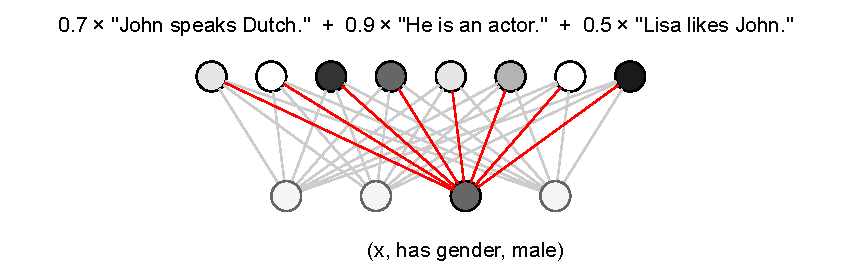
\includegraphics{4_approach/1_texter/2_attention_model/multi_linear}
    \caption{Multi-linear}
    \label{fig:4_approach/1_texter/2_attention_model/multi_linear}
\end{figure}

Similar to the simple Texter, following the core steps, the attentive Texter takes all classes whose confidences, that result from applying the sigmoid function to the output logits, is greater than 50\% to form their corresponding facts and sort them by confidence. In addition to the simple Texter, however, the attentive model provides the facts with the sentence weights as they result from the attention matrix in order to provide the user with an explanation for each fact's prediction. So, in the example, the fact $(John, has~gender, male)$, with a probability around 70\%, would be accompanied by the information that it was primarily suggested due to the sentence "He is an actor.", followed by "John speaks Dutch." and lastly "Lisa likes John.".

learnable class embs
sigmoid maps to (0, 1)
attention matrix A
total number of learnable params
in experiments: applied by an AdamW optimizer, a variant of the Adam optimizer that overcomes Adam's that keeps the training speed of Adam while keeping SGD's superior ability to generalize~, \cite{Loshchilov2019DecoupledWD}




\section{Ruler}
\label{sec:4_approach/2_ruler}
While the Texter processes the text information attached to the knowledge graph's entities, the Ruler exploits patterns in the graph structure to predict missing facts. Given an entity $x$ with a set of known facts $K$ containing facts of the form $(x, rel_k, tail_k)$ with $1 <= k <= |K|$ and $rel_k \in R$ and $tail_k \in E$ being any relation or entity, respectively, the Ruler leverages entity-related rules of the form $(x, rel_m, tail_m) <= (x, rel_k, tail_k)$ with $1 <= m <= |M|$ to predict a set of missing facts $M$. Therefore, the rules required for the inference process have to be mined from the knowledge graph, beforehand. That rule mining process can be viewed as the equivalent to the Texter's training process and some paragraphs in this thesis will refer to combined rule mining and creation of a Ruler as "training" a Ruler. Compatibel to the Texter, the Ruler is limited to the prediction of facts $(x, rel, tail)$ that contain the query entity as their head, as well. However, when the Ruler is applied to all entities $e \in E$, all facts of the form $(e, rel, x)$ are predicted at some point as far as the mined rules support it.

For rule mining, AnyBURL, the bottom-up rule mining algorithm, by Christian Meilicke et al.~\cite{Meilicke2019AnytimeBR} is used. It is an anytime algorithm, meaning that it can be interrupted anytime and still yield valid results. Bottom-up rule mining refers to the fact that the algorithm starts with concrete paths in the graph and tries to generalize those paths to rules instead of coming up with rules initially and searching for evidence later, which would be a top-down approach. Out of all possible Horn rules that might describe patterns in the graph, AnyBURL is restricted to rules that can be generalized from so-called \emph{ground path rules}. A ground path rule does not contain variables, but only constants, and must not contain any cycles in its body. Equation~\ref{eq:4_approach/2_ruler/ground_path_rule} describes the general form of a ground path rule of length $n$, meaning that it consists out of the head fact and $n$ body facts.

\begin{align}
(c_0, h, c_1)
    \Leftarrow (c_1, b_1, c_2), \dots, (c_n, b_n, c_{n+1}) &&
    c_k \neq c_l \forall k, l \in \{1, \dots, n+1\}, k \ne l
    \label{eq:4_approach/2_ruler/ground_path_rule}
\end{align}

Notably, despite the rule body being free of cycles, the ground path rule as a whole can still be cyclic if $c_0 = c_{n+1}$. Ground path rules are derived directly from randomly sampled paths in the graph and are subsequently generalized to rules that replace some of the constants with variables. If further supporting paths can be found for a general rule, it is kept. In their paper on AnyBURL, Meilicke et al. show that any rule that can be generalized from a ground path rules can be generalized to one of the three rule types formulated in Equations~\ref{eq:4_approach/2_ruler/c}~--~\ref{eq:4_approach/2_ruler/ac2}. Thereby, $C$-type rules can only be generalized from cyclic ground path rules, $AC2$ rules can only be generalized from acyclic ground path rules and $AC1$ can be generalized from both, cyclic and acyclic ground path rules. The following paragraphs outline the core algorihm used to mine such rules and derive some example rules from the small graph introduced in Chapter~\ref{ch:1_introduction}. Figure~\ref{fig:4_approach/2_ruler/rule_graph} shows an annotated subset of the graph that illustrates the rules. "Amsterdam" and "Netherlands" have been abbreviated to "AMS" and "NL" to keep the examples short.

\begin{align}
    C   && (Y, h, X)   &\Leftarrow (X, b_1, A_2), \dots, (A_n, b_n, Y)
    \label{eq:4_approach/2_ruler/c} \\
    AC1 && (c_0, h, X) &\Leftarrow (X, b_1, A_2), \dots, (A_n, b_n, c_{n+1})
    \label{eq:4_approach/2_ruler/ac1} \\
    AC2 && (c_0, h, X) &\Leftarrow (X, b_1, A_2), \dots, (A_n, b_n, A_{n+1})
    \label{eq:4_approach/2_ruler/ac2}
\end{align}

\begin{figure}[t]
    \centering
    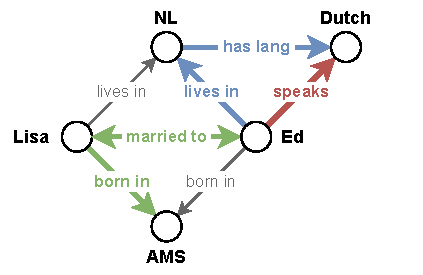
\includegraphics{4_approach/2_ruler/rule_graph}
    \caption{Subset of the previously introduced example graph with highlighted facts that form an acyclic (red + green) and a cyclic (red + blue) path.}
    \label{fig:4_approach/2_ruler/rule_graph}
\end{figure}

Essentially, AnyBURL repeatedly samples random paths from the graphs, generalizes them to all possible rule types, looks for further paths that match the gained rules, and keeps those rules it finds further evidence for. For example, in search of rules of length 2, i.e. rules that have a body consisting of 2 facts, AnyBURL might randomly sample the two paths in~\ref{eq:4_approach/2_ruler/path_1} and~\ref{eq:4_approach/2_ruler/path_2} from the graph. Note, that parentheses denote entities, brackets denote relations and that the path does not need to follow directed edges in the graph. Furthermore, a close look at the paths reveals that the second path is cyclic as it starts and ends at the entity "Dutch".

\begin{align}
(Dutch)
    \leftarrow [speaks] - (Ed) - [married~to] \rightarrow (Lisa) - [born~in] \rightarrow (AMS)
    \label{eq:4_approach/2_ruler/path_1} \\
    (Dutch) \leftarrow [speaks] - (Ed) - [lives~in] \rightarrow (NL) - [has~lang] \rightarrow (Dutch)
    \label{eq:4_approach/2_ruler/path_2}
\end{align}

From those paths, AnyBURL would then derive the constant-only
ground path rules~\ref{eq:4_approach/2_ruler/acyclic_ground_path} and~\ref{eq:4_approach/2_ruler/cyclic_ground_path} by taking the path's first part as the rule's head and the remaining parts to form the rule's body.

\begin{align}
(Ed, speaks, Dutch)
    &\Leftarrow (Ed, married~to, Lisa), (Lisa, born~in, AMS)
    \label{eq:4_approach/2_ruler/acyclic_ground_path} \\
    (Ed, speaks, Dutch) &\Leftarrow (Ed, lives~in, NL), (NL, has~lang, Dutch)
    \label{eq:4_approach/2_ruler/cyclic_ground_path}
\end{align}

The acyclic ground path rule in~\ref{eq:4_approach/2_ruler/acyclic_ground_path} can be generalized to the $AC1$ rule~\ref{eq:4_approach/2_ruler/acyclic_ac1} and the $AC2$ rule~\ref{eq:4_approach/2_ruler/acyclic_ac2} while the cyclic ground path rule~\ref{eq:4_approach/2_ruler/cyclic_ground_path} can be generalized to the $C$ rule~\ref{eq:4_approach/2_ruler/cyclic_c} and the $AC1$ rule~\ref{eq:4_approach/2_ruler/cyclic_ac1}.

\begin{align}
    AC1 && (X, speaks, Dutch) &\Leftarrow (X, married~to, A_2), (A_2, born~in, AMS)
    \label{eq:4_approach/2_ruler/acyclic_ac1} \\
    AC2 && (X, speaks, Dutch) &\Leftarrow (X, married~to, A_2), (A_2, born~in, A_3)
    \label{eq:4_approach/2_ruler/acyclic_ac2} \\
        C   && (X, speaks, Y) &\Leftarrow (X, lives~in, A_2), (A_2, has~lang, Y)
    \label{eq:4_approach/2_ruler/cyclic_c} \\
    AC1 && (X, speaks, Dutch) &\Leftarrow (X, lives~in, A_2), (A_2, has~lang, Dutch)
    \label{eq:4_approach/2_ruler/cyclic_ac1}
\end{align}

Next, every rule candidate is scored by looking for further paths that match the rule's body and checking whether the graph also contains the fact predicted by the rule, i.e. whether the rule is correct in that case. Thereby, the number of paths that match the rule body is called the rule's \emph{support} while the ratio of times the rule is correct over its total support is called \emph{confidence}. Taking the cyclic rule~\ref{eq:4_approach/2_ruler/cyclic_c} as an example, AnyBURL would search for further evidence and find the path $(Lisa) - [lives~in] -> (NL) - [has~lang] -> (Dutch)$ that matches the rule body, increasing the rule's support to two, so far. However, the example graph does not contain the rule's predicted fact $(Lisa, speaks, Dutch)$, so the rule's support drops from 1 to $\frac{1}{2}$. Since rules that only apply to a single case or only once in every thousands case are not very useful, AnyBURL drops rules with a support of 1 or confidence below 0.0001 by default~\cite{AnyBURL}. It is noteworthy that, although some rules are more general than others, such as~\ref{eq:4_approach/2_ruler/acyclic_ac2} compared to~\ref{eq:4_approach/2_ruler/acyclic_ac1}, the more specific ones are still kept as they might end up with higher confidence for their special case during the ongoing mining process.

The process described by the above example is repeated until only few new rules of the same length $n$ can be found. AnyBURL then continues its search for rules of length $n + 1$ until it terminates after a fixed number of time steps. Listing~\ref{code:anyburl} shows the slightly adjusted pseudocode from the AnyBURL paper. The sampling and scoring process discussed above is implemented as the body of the inner while loop. The outer for loop implements the repeated check for the saturation of rules of the current length and the eventual proceeding to rules of increased length.

% TODO param s

\begin{listing}[t]
    \begin{lstlisting}
        AnyBURL(G, sat, Q, i, ts):
            n = 2
            R = $\emptyset$
            for i times:
                $R_s = \emptyset$
                start = current_time()
                while current_time() < start + ts:
                    p = sample_path(G, n)
                    $R_p$ = generate_rules(p)
                    for $r$ in $R_p$:
                        score($r$)
                        if $Q$($r)$:
                            $R_s$ = $R_s \cup {r}$

                $R_s^{'}$ = $R_s \cap R$
                if $|R_s^{'}| / |R_s| > sat$:
                    n = n + 1
                $R$ = $R \cup R_s$

            return $R$
    \end{lstlisting}
    \caption{The AnyBURL rule mining algorithm takes a graph $G$, a saturation level $sat$, a quality criterion $Q$, and a number of iterations $i$, each of a timespan $ts$, as input and produces a ruleset $R$.}
    \label{code:anyburl}
\end{listing}

A walk through the pseudocode reads as follows: Given the Graph $G$, the saturation threshold $s$, the quality criterion $Q$, a number of iterations $i$ and the timespan $ts$ each iteration endures, AnyBURL starts with an empty ruleset $R$, that will be extended after each iteration and returned in the end. The initial length of the randomly sampled paths is $n=2$, allowing to find the shortest possible rules of length 1. During the first iteration of duration $ts$, AnyBURL fills the rule set $R_s$, that keeps the rules found in the current iteration, by repeatedly sampling paths, generating rules from the paths, scoring the resulting rules, and keeping those with sufficient support and confidence. At the end of the iteration, when the timespan $ts$ has passed, $R_s^{'}$ is calculated as the set of rules mined during the iteration that were already known. If the share of already known rules mined during the current iteration exceeds the saturation threshold, the algorithm starts searching for rules of increased length. Otherwise, it continues with the current length. In both cases, the iteration's rules are added to the overall ruleset $R$. If the specified number of total iterations is reached, AnyBURL terminates and returns the mined rules $R$. In practice, AnyBURL saves the mined rules in a text file at the end and at configurable points during mining.

With the stored rules from AnyBURL in place, the Ruler is prepared for inference. Conceptually, given an entity and its known facts, the Ruler loads the rules, filters out further rules that do not meet the Ruler's quality demands and applies the remaining, useful rules to all known facts. All rules that can be applied successfully are kept together with their confidence. From all the facts predicted by the applied rules, already known facts from the existing graph are filtered out. The remaining facts are sorted by confidence and returned to the user - together with the rules that predicted them as an explanation for the user. If multiple rules predict the same fact, the fact is assigned the highest confidence of those rules and is returned together with all of them. The Ruler's extra quality criterion mentioned above further restricts the considered rules to those with confidence greater 50\%, because AnyBURL's minimum confidence threshold of 0.01\% allows many rules that predict false positives. For open-world entities, this algorithm implies an empty result set as no rule can cover an entity that is not connected to any other entity and all the facts predicted for the train entities will be filtered out. In those cases, the Power model has to rely solely on the Texter.



\section{Aggregator}
\label{sec:4_approach/3_aggregator}
The aggregator has the task of merging the predicted facts from Ruler and Texter. As envisioned in \autoref{sec:4_approach/3_aggregator} and illustrated in \autoref{fig:4_approach/3_aggregator/lucy}, it was hoped that merging the facts leads to higher average precision because facts predicted by both components are likely to be correct and should be ranked higher. In addition, the Aggregator should be able to estimate how reliable the predictions of Ruler and Texter are in relation to each other, which is implemented in the form of the weight parameter $\alpha$ as described in \autoref{eq:4_approach/3_aggregator/conf_aggregator}.

\autoref{tab:5_experiments/5_aggregator/results} shows the final evaluation results for the Aggregator, and thus the final evaluation results for the Power model, for a number of graph-text combinations. As fact splits, the splits with 50\% known test facts were chosen, as for the final Ruler evaluation in \autoref{sec:5_experiments/4_ruler}. The respective results for the CDE-50 and FB-50 splits from \autoref{tab:5_experiments/4_ruler/results} were taken over into \autoref{tab:5_experiments/5_aggregator/results} for easier comparability. Similarly, the chosen text sets are the ones from the final Texter evaluation in \autoref{subsec:5_experiments/3_texter/3_context}. Again, \autoref{tab:5_experiments/5_aggregator/results} duplicates the respective results from \autoref{tab:5_experiments/3_texter/3_context/results} for ease of comparison. The last two columns then contain the new Aggregator measurements for the combination of the corresponding Ruler and Texter.

\begin{table}[t]
    \makebox[\textwidth][c]{
        \begin{tabular}{ l l c r r r }
    \toprule

    \multicolumn{1}{l}{\textbf{Text Set}} &
    \multicolumn{1}{l}{\textbf{Texter}} & \phantom &
    \multicolumn{3}{c}{\textbf{Macro over Classes}} \\

    \cmidrule{4-6}

    & 
    &&
    \multicolumn{1}{c}{\textbf{Prec}} &
    \multicolumn{1}{c}{\textbf{Rec}} &
    \multicolumn{1}{c}{\textbf{F1}} \\
    
    \midrule

    \multirow{2}{*}{cde-cde-1-clean}
    & Simple    && \textbf{49.02} & 47.57 & 47.67 \\
    & Attentive && 46.86 & \textbf{51.09} & \textbf{47.98} \\

    \addlinespace

    \multirow{2}{*}{cde-irt-1-clean}
    & Simple    && 25.20 & \textbf{34.18} & \textbf{28.13} \\
    & Attentive && \textbf{26.70} & 31.41 & 27.43 \\

    \addlinespace

    \multirow{2}{*}{cde-irt-5-clean}
    & Simple    && 36.49 & \textbf{44.38} & \textbf{38.98} \\
    & Attentive && \textbf{39.20} & 37.11 & 36.98 \\

    \addlinespace

    \multirow{2}{*}{cde-irt-15-clean}
    & Simple    && 41.83 & \textbf{48.69} & \textbf{44.07} \\
    & Attentive && \textbf{44.63} & 37.39 & 39.78 \\

    \addlinespace

    \multirow{2}{*}{cde-irt-30-clean}
    & Simple    && 40.73 & \textbf{50.09} & \textbf{44.11} \\
    & Attentive && \textbf{43.60} & 36.10 & 38.78 \\
    
    \midrule

    \multirow{2}{*}{fb-owe-1-clean}
    & Simple    && 42.36 & \textbf{86.72} & 54.03 \\
    & Attentive && \textbf{45.21} & 84.03 & \textbf{56.16} \\

    \addlinespace

    \multirow{2}{*}{fb-irt-1-clean}
    & Simple    && 26.40 & 46.68 & 32.51 \\
    & Attentive && \textbf{27.01} & \textbf{49.90} & \textbf{34.26} \\

    \addlinespace

    \multirow{2}{*}{fb-irt-5-clean}
    & Simple    && 34.37 & \textbf{55.95} & 40.88 \\
    & Attentive && \textbf{39.21} & 50.63 & \textbf{43.50} \\

    \addlinespace

    \multirow{2}{*}{fb-irt-15-clean}
    & Simple    && \textbf{48.95} & \textbf{54.85} & \textbf{50.06} \\
    & Attentive && 48.89 & 52.75 & 49.92 \\

    \addlinespace

    \multirow{2}{*}{fb-irt-30-clean}
    & Simple    && 43.90 & \textbf{63.31} & \textbf{50.55} \\
    & Attentive && \textbf{50.57} & 48.47 & 48.79 \\
    
    \bottomrule
\end{tabular}

    }
    \caption{Final Aggregator results, i.e. final results for the Power model. The results of the Ruler and Texter, whose predictions the Aggregator combines, are also shown for comparison. Although the Aggregator does not outperform its respective Ruler and Texter in terms of F1 score, it does for mAP.}
    \label{tab:5_experiments/5_aggregator/results}
\end{table}

As the mAP values show, the Aggregator performs several percentage points better than the Ruler and Texter on their own, with the improvement on the CDE split being more obvious. However, the relatively small increase on the FB split suggests that the true positives of Ruler and Texter almost coincide there. For the CDE split, on the other hand, manually peeking into the predictions reveals that the improved mAP mainly results from complementary true positives -- and not so much from improved ranks of joint predictions. Looking at the values of simple and attentive Texter, it is also noticeable that the lead of the simple Texter over the attentive Texter shrinks when adding the Ruler. Likewise, the lead of the text sets with many sentences and with high-quality sentences shrinks. Finally, the different aptitudes for Ruler and Overall, the Aggregator results are even similar between the two splits, while previously, models performed significantly better on the FB split.

Two experiments that will be mentioned only briefly here, because of their unspectacular results, concerning the calculation of the Aggregator's confidence as per \autoref{eq:4_approach/3_aggregator/conf_aggregator}: First, in the beginning, experiments were conducted on the computation of the combined confidence $conf_{Aggregator}$ in cases where facts are predicted by Ruler and Texter. As combining methods, calculating the maximum and the mean of $conf_{Ruler}$ and $conf_{Texter}$ were evaluated, but it soon became apparent that summing them up much better accommodates the fact that a fact predicted by Ruler and Texter deserves very high confidence. Second, experiments showed that taking into account the weight parameter $\alpha$ between Ruler and Texter yields only marginal performance improvements in the tenths of a percent range because the confidence values of Ruler and Texter seem to be very comparable after all and thus always yield $\alpha$ values close to 0.5. In detail, Ruler and Texer were both a bit too optimistic about their predictions in the experiments -- but they were equally overconfident.

